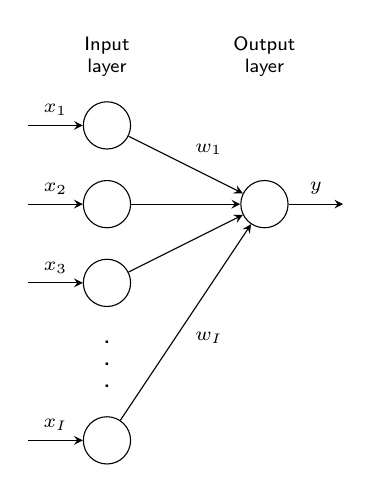
\begin{tikzpicture}[x=1.0cm, y=1.0cm, >=stealth, font=\sffamily\scriptsize]
    \tikzstyle{every neuron}=[circle, draw, minimum size=.6cm]
    \tikzstyle{neuron missing}=[draw=none, scale=2, text height=0.333cm, execute at begin node={\color{black}\tiny$\vdots$}]
    
    % Input nodes
    \foreach \m/\l [count=\y] in {1,2,3,missing,4}
        \node [every neuron/.try, neuron \m/.try] (input-\m) at (0,2.5-\y) {};
      
    % Output node
    \node [every neuron/.try, neuron 1/.try ] (output-1) at (2,1.5-1) {};

    % Names on input arrows
    \foreach \l [count=\i] in {1,2,3,I}
        \draw [<-] (input-\i) -- ++(-1,0) node [above, midway] {$x_\l$};
    
    % Name on output arrow
    \draw [->] (output-1) -- ++(1,0) node [above, midway] {$y$};
    
    % Inputs -> Outputs
    \draw [->] (input-1) -- node[above right]{$w_{1}$} (output-1);
    \draw [->] (input-2) -- (output-1);
    \draw [->] (input-3) -- (output-1);
    \draw [->] (input-4) -- node[below right]{$w_{I}$} (output-1);
    
    % Layer names
    \foreach \l [count=\x from 0] in {Input\\layer, Output\\layer}
        \node [align=center, above] at (\x*2,2) {\l};
\end{tikzpicture}